% =====================================================================
\section{Supplementary scans and diagnostics}
\label{app:supp}

This appendix collects the parameter scans, ablations and
diagnostics that justify the configuration choices reported in
Sec.~\ref{sec:results}.

\subsection{Inverse PINN: template diagnostics}
\label{app:supp-inv}

Tables~\ref{tab:inv-learned} and~\ref{tab:tau-degeneracy} list
the learned template scalars for the six inverse variants and
compare $\tau_{\mathrm{learned}}$ with the post-hoc M2
wide-window fit: the strongly template-weighted variants (A, D,
E) drift $1.2$--$1.9\,M$ below the post-hoc value along the
$A_{\mathrm{ring}}$--$\tau$ degeneracy of
Eq.~\eqref{eq:loss-ring} while the field retains the physical
decay rate --- the quantitative basis for the reporting
convention of Sec.~\ref{sec:reporting}.

\begin{table}[!htbp]
\centering
\caption{Inverse PINN learned template parameters at the end of
training for each
variant. These are the values of the learnable scalars
$(\omega,\tau,A_{\mathrm{ring}},\phi)$ inside the ringdown loss of
Eq.~\eqref{eq:loss-ring} after $10{,}000$ Adam plus $15{,}000$
L-BFGS iterations. They are reported as a diagnostic and are not
the primary QNM estimates of Table~\ref{tab:inv-summary}; the
reason is given in the
$A_{\mathrm{ring}}$--$\tau$ paragraph below.}
\label{tab:inv-learned}
\small
\begin{tabular}{@{}lcccc@{}}
\toprule
Variant & $\omega_{\mathrm{learned}}$ & $\tau_{\mathrm{learned}}/M$ &
        $A_{\mathrm{ring}}$ & $\phi$ \\
\midrule
baseline   & $0.3820$ & $11.89$ & $1.92$ & $-0.99$ \\
A          & $0.3704$ & $10.10$ & $2.59$ & $-0.72$ \\
B          & $0.4050$ & $8.62$  & $2.97$ & $-1.38$ \\
C          & $0.3822$ & $11.84$ & $1.92$ & $-0.99$ \\
D          & $0.3748$ & $9.48$  & $2.93$ & $-0.85$ \\
E (mode 0) & $0.3496$ & $9.22$  & $2.52$ & $+0.31$ \\
E (mode 1) & $0.3810$ & $7.38$  & $3.24$ & $-1.90$ \\
\bottomrule
\end{tabular}
\end{table}

\begin{table}[!htbp]
\centering
\caption{$A_{\mathrm{ring}}$--$\tau$ degeneracy diagnostic. The
training-time learned $\tau_{\mathrm{learned}}$ is the value of the
learnable scalar at the end of training. The post-hoc M2 wide-window
$\tau_{\mathrm{M2}}^{\mathrm{wide}}$ is the M2 fit to
$\Phi_\theta(\xq,t)$ over $[10,50]\,M$. Truth is
$\tau_0/M = 11.241$ \citep{Leaver1985}. ``Bias gap'' is
$|\tau_{\mathrm{learned}} - \tau_{\mathrm{M2}}^{\mathrm{wide}}|/M$.
For variant E, $\tau_{\mathrm{learned}}$ refers to the fundamental
template mode (mode 0).}
\label{tab:tau-degeneracy}
\small
\begin{tabular}{@{}lccc@{}}
\toprule
Variant & $\tau_{\mathrm{learned}}/M$ & $\tau_{\mathrm{M2}}^{\mathrm{wide}}/M$ & Bias gap \\
\midrule
baseline & $11.89$ & $11.83$ & $0.06$ \\
A        & $10.10$ & $11.29$ & $1.19$ \\
B        & $8.62$  & $8.63$  & $0.01$ \\
C        & $11.84$ & $11.82$ & $0.02$ \\
D        & $9.48$  & $11.06$ & $1.58$ \\
E        & $9.22$  & $11.10$ & $1.88$ \\
\bottomrule
\end{tabular}
\end{table}

\subsection{Hybrid: gradient-gate diagnostics}
\label{app:supp-gate}

Figure~\ref{fig:hyb-grad} shows the per-cell scatter of
coarse-prior error against prior gradient magnitude on the
canonical BH (log--log Pearson $r = 0.917$), the empirical
basis of the gradient gate, and
Table~\ref{tab:hyb-gate-decile} the decile stratification: the
gated correction reduces the mean error by $14.1\times$ in the
top gradient decile, declining monotonically to $2.6\times$ in
the sixth, with the sub-median cells left at the prior floor.
The gate scale itself is fixed label-free in
Appendix~\ref{app:gate-scale}.

\begin{figure}[!htbp]
\centering
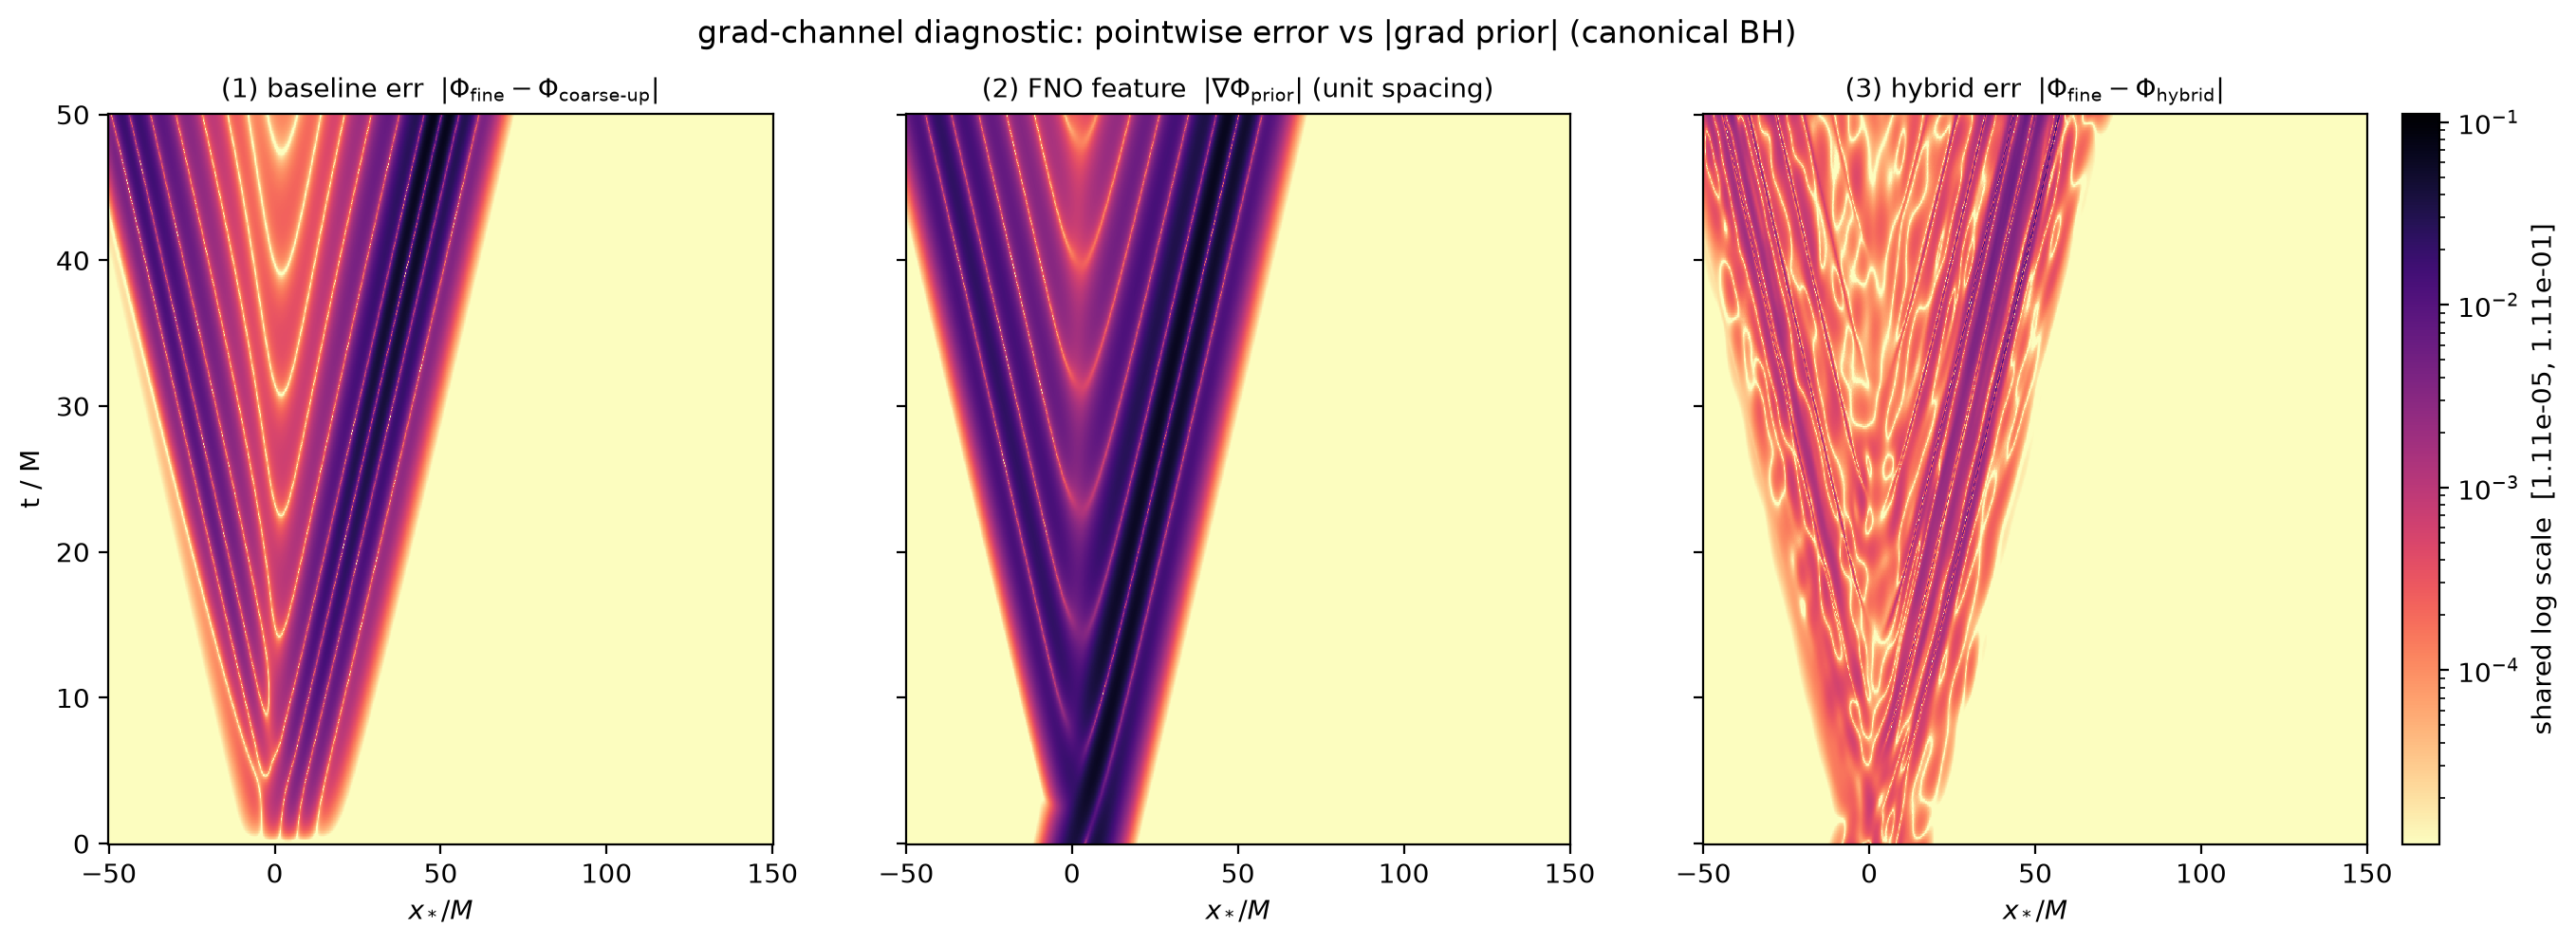
\includegraphics[width=0.82\textwidth]{../outputs/hybrid/fno_sw_gate_s1em3/figs/grad_vs_error.png}
\caption{Coarse-prior error versus prior gradient on the
canonical BH, the diagnostic motivating the gradient gate.
Each point is one $(x,t)$ cell; the horizontal axis is the
prior gradient magnitude $|\nabla\mathcal{U}\Phi^{\mathrm{c}}|$
and the vertical axis the coarse-up baseline error
$|\Phi^{\mathrm{f}} - \mathcal{U}\Phi^{\mathrm{c}}|$, both on
log scales. The log--log Pearson correlation is $r = 0.917$:
the prior error is large precisely on the high-gradient
wavefronts and small in the low-gradient interior and causal
exterior, so the gate $g$ (Eq.~\eqref{eq:hyb-gate}) routes the
network correction to the cells that need it.}
\label{fig:hyb-grad}
\end{figure}

\begin{table}[!htbp]
\centering
\caption{Hybrid error reduction stratified by coarse-prior
gradient on the canonical BH. Cells are sorted into deciles of
$|\nabla\mathcal{U}\Phi^{\mathrm{c}}|$; for the top four
deciles (the wavefront-bearing cells) the table lists the
decile-mean gradient, the mean coarse-up baseline error, the
mean hybrid error, and their ratio. Below the median the prior
gradient is $\lesssim 10^{-12}$ (smooth interior and causal
exterior) and both errors are at the field floor.}
\label{tab:hyb-gate-decile}
\small
\setlength{\tabcolsep}{6pt}
\begin{tabular}{@{}lcccc@{}}
\toprule
Gradient decile & $\overline{|\nabla\mathcal{U}\Phi^{\mathrm{c}}|}$
 & baseline err & hybrid err & ratio \\
\midrule
90--100\% (wavefronts) & $3.15\times 10^{-2}$ & $1.30\times 10^{-2}$ & $9.22\times 10^{-4}$ & $14.1$ \\
80--90\%               & $1.01\times 10^{-2}$ & $4.37\times 10^{-3}$ & $4.42\times 10^{-4}$ & $9.9$  \\
70--80\%               & $3.56\times 10^{-3}$ & $2.21\times 10^{-3}$ & $2.58\times 10^{-4}$ & $8.6$  \\
60--70\%               & $4.37\times 10^{-4}$ & $6.81\times 10^{-4}$ & $2.60\times 10^{-4}$ & $2.6$  \\
\bottomrule
\end{tabular}
\end{table}

\subsection{Hybrid M5 plateau diagnostic}
\label{app:supp-m5}

Figure~\ref{fig:hyb-plateau-m5}
shows the M5 2-D plateau scan for the hybrid canonical
extraction; it confirms the main-text M4 value
(Table~\ref{tab:hyb-canonical}).

\begin{figure}[!htbp]
\centering
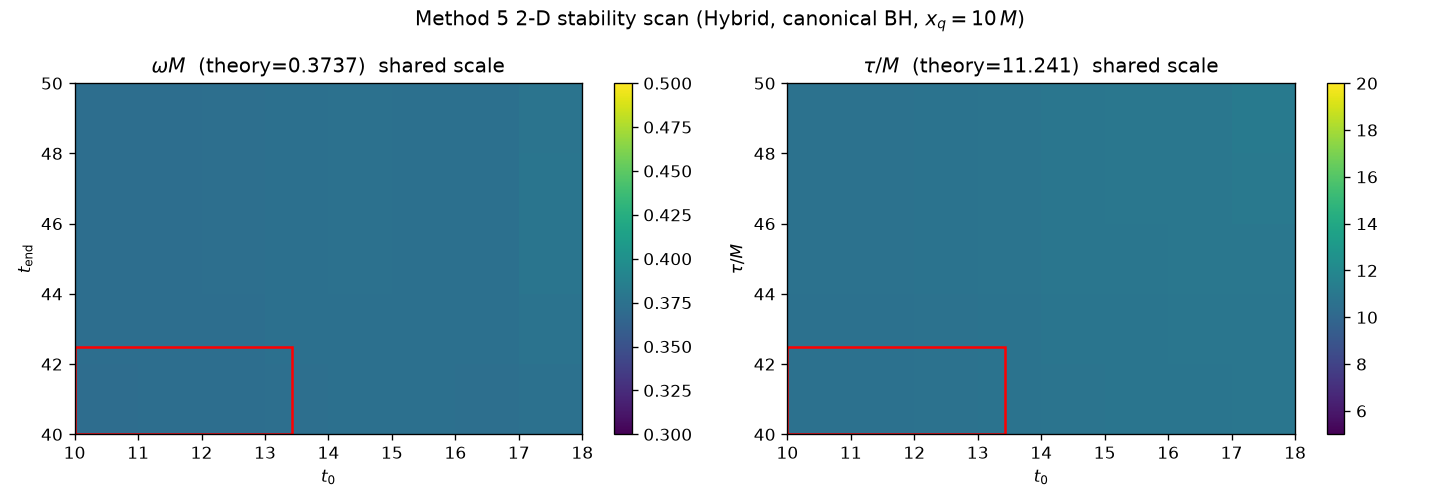
\includegraphics[width=0.95\textwidth]{../outputs/hybrid/fno_sw_gate_s1em3/figs/hybrid_plateau_m5_xq10.png}
\caption{M5 2-D plateau scan on the hybrid prediction at the
canonical BH and $\xq = 10\,M$. Heatmaps of the fitted
$\omega$ (left) and $\tau$ (right) over an $8 \times 5$ grid in
$(t_{0}, \tend)$ with $t_{0} \in [10, 18]\,M$ and
$\tend \in [40, 50]\,M$, on the shared colour scales
$\omega \in [0.30, 0.50]$ and $\tau \in [5, 20]\,M$. The red
rectangle marks the identified plateau block
($t_{0} \in [10.0, 13.4]\,M$,
$\tend \in [40.0, 42.5]\,M$). White cells are NLS fits that
failed to converge.}
\label{fig:hyb-plateau-m5}
\end{figure}
